\documentclass[../thesis.tex]{subfiles}
\graphicspath{{\subfix{../assets/}}}
\begin{document}

\chapter{Perceptually Aligned Gradients}
In the context of image classifiers, adversarially robust models show up Perceptually Aligned Gradients, also PAG for short \citep{engstrom2019adversarialpag} \citep{Ross_Doshi-Velez_2018_pag}.
They are a characteristic that allow the gradients of the loss with respect to the input sample to be perceived by humans as having something in common with the actual identified class.
For instance, by simply observing a gradient image created as
$\nabla_x \mathcal{L}(x; y = \text{dog}) \in \mathbb{R}^3 \;\text{s.t.}\; x \in C_{\text{dog}} $,
it can be perceived of having some dog's features, such as the overall shape or the muzzle of the animal.
This means that a robust classifier is by far more interpretable, since it is possible to see the learnt main features.
In the case of targeted attacks, they generally require adding a perturbation to the image that is so intrusive that almost reconstructs the features of the targeted class, making the overall attack perceptible by a human operator, thus nullifying its stealth effect \citep{aggarwal2020benefitspag}.

Later on, \citeauthor{pag-imply-robustness} questioned whether having a classifier trained with a PAG objective in the loss function would make it manifest some features unique of robust classifiers.
In this specific scenario, the loss function of a classifier would be:

\begin{equation}
\label{eq:pag_image_training_formula}
\begin{split}
\mathcal{L}(x, y) = \mathcal{L}_{CE}( f_\theta(x), y)
                + \lambda \frac{1}{C} \sum_{y_t=1}^C \mathcal{L}_{cos}(\nabla_x f_\theta(x)_{y_t}, g(x, y_t))
\end{split}
\end{equation}

The standard cross-entropy loss is combined with the regularization term given by the gradients alignment with $g(x, y_t)$.
The cosine loss is essentially the inverse of the cosine similarity as it is usually defined.

\begin{equation}
\mathcal{L}_{cos}(\mathbf{v}, \mathbf{u}) = 1 - sim_{cos}(\mathbf{v}, \mathbf{u})
\end{equation}

\section{PAG applied to a sentence classifier}
It is not feasible to naively apply the PAG regularized training in formula \cref{eq:pag_image_training_formula} to a LLM:
even by considering a LLM as a next-token classifier, it would present way too many classes (as many as the vocabulary size $|V|$) to optimize, but also there is not a clear meaning of what the common features of all the prefixes that predict a certain continuation token should be.
Moreover, there is a serious risk of wasting computational resources approaching a problem so big directly.

Instead, we plan to proceed by small steps.
In this first experiment, a binary sentence classifier is built to predict, given the DistilBERT
\footnote{\url{https://huggingface.co/distilbert/distilbert-base-cased}}
embeddings of a sentence, whether it is a positive or negative review, leveraging the sentiment analysis IMDB dataset from HuggingFace.
\footnote{\url{https://huggingface.co/datasets/stanfordnlp/imdb}}
The sentence embeddings are obtained taking the hidden state of the last layer, with respect to the \texttt{[CLS]} start token, resulting in a vector embedding $\mathbf{e} \in \mathbb{R}^{768}$.
Additionally, in this setting, it is possible to make the training process tremendously faster by precomputing and storing the sentence embeddings once and for all, skipping the DistilBERT inference at each training step.

The ground-truth gradient is defined by the function $g(x, y_t)$.
Several strategies may be used to compute it, but in our experiment we are using the following formulation:
\begin{equation}
    \label{eq:pag_bce_imdb_sentiment_analysis}
    g(x, y) = u_y - x \quad\text{s.t.}\; u_y \in C_y \;\wedge\; u_y \neq x
\end{equation}

The ground-truth gradient image is computed as the difference between the current sample $x$ and a random sample $u_y$, different from $x$, of class $y$. Note that $x$ may not be of class $y$ as well, since in the full loss (\cref{eq:pag_image_training_formula}) $g(x, y)$ is called for each $y$, independently of the ground-truth class of $x$.

The \textbf{baseline} classifier is a feed-forward neural network, that works on the same training split, hyper-parameter values and model architecture. The only difference is in the loss function: the baseline is training using only the standard binary cross-entropy loss.

\subsubsection{Overfitting regularization}
We can see that the cosine similarity between $x$ and $\nabla_x \mathcal{L}(x;y)$ went from almost between $-0.1$ and $0$ in the baseline model, indicating an absence of correlation, to a strongly positive value reaching almost $0.5$ highlighting a positive correlation.

It is worth mentioning that the baseline converged much quicker than the PAG-regularized model,
since the latter took $\approx 8\times$ the number of epochs to also let the regularization loss ($\mathcal{L}_{cos}$) reach low amounts.

\begin{figure}
    \centering
    \begin{subfigure}{0.48\linewidth}
        \centering
        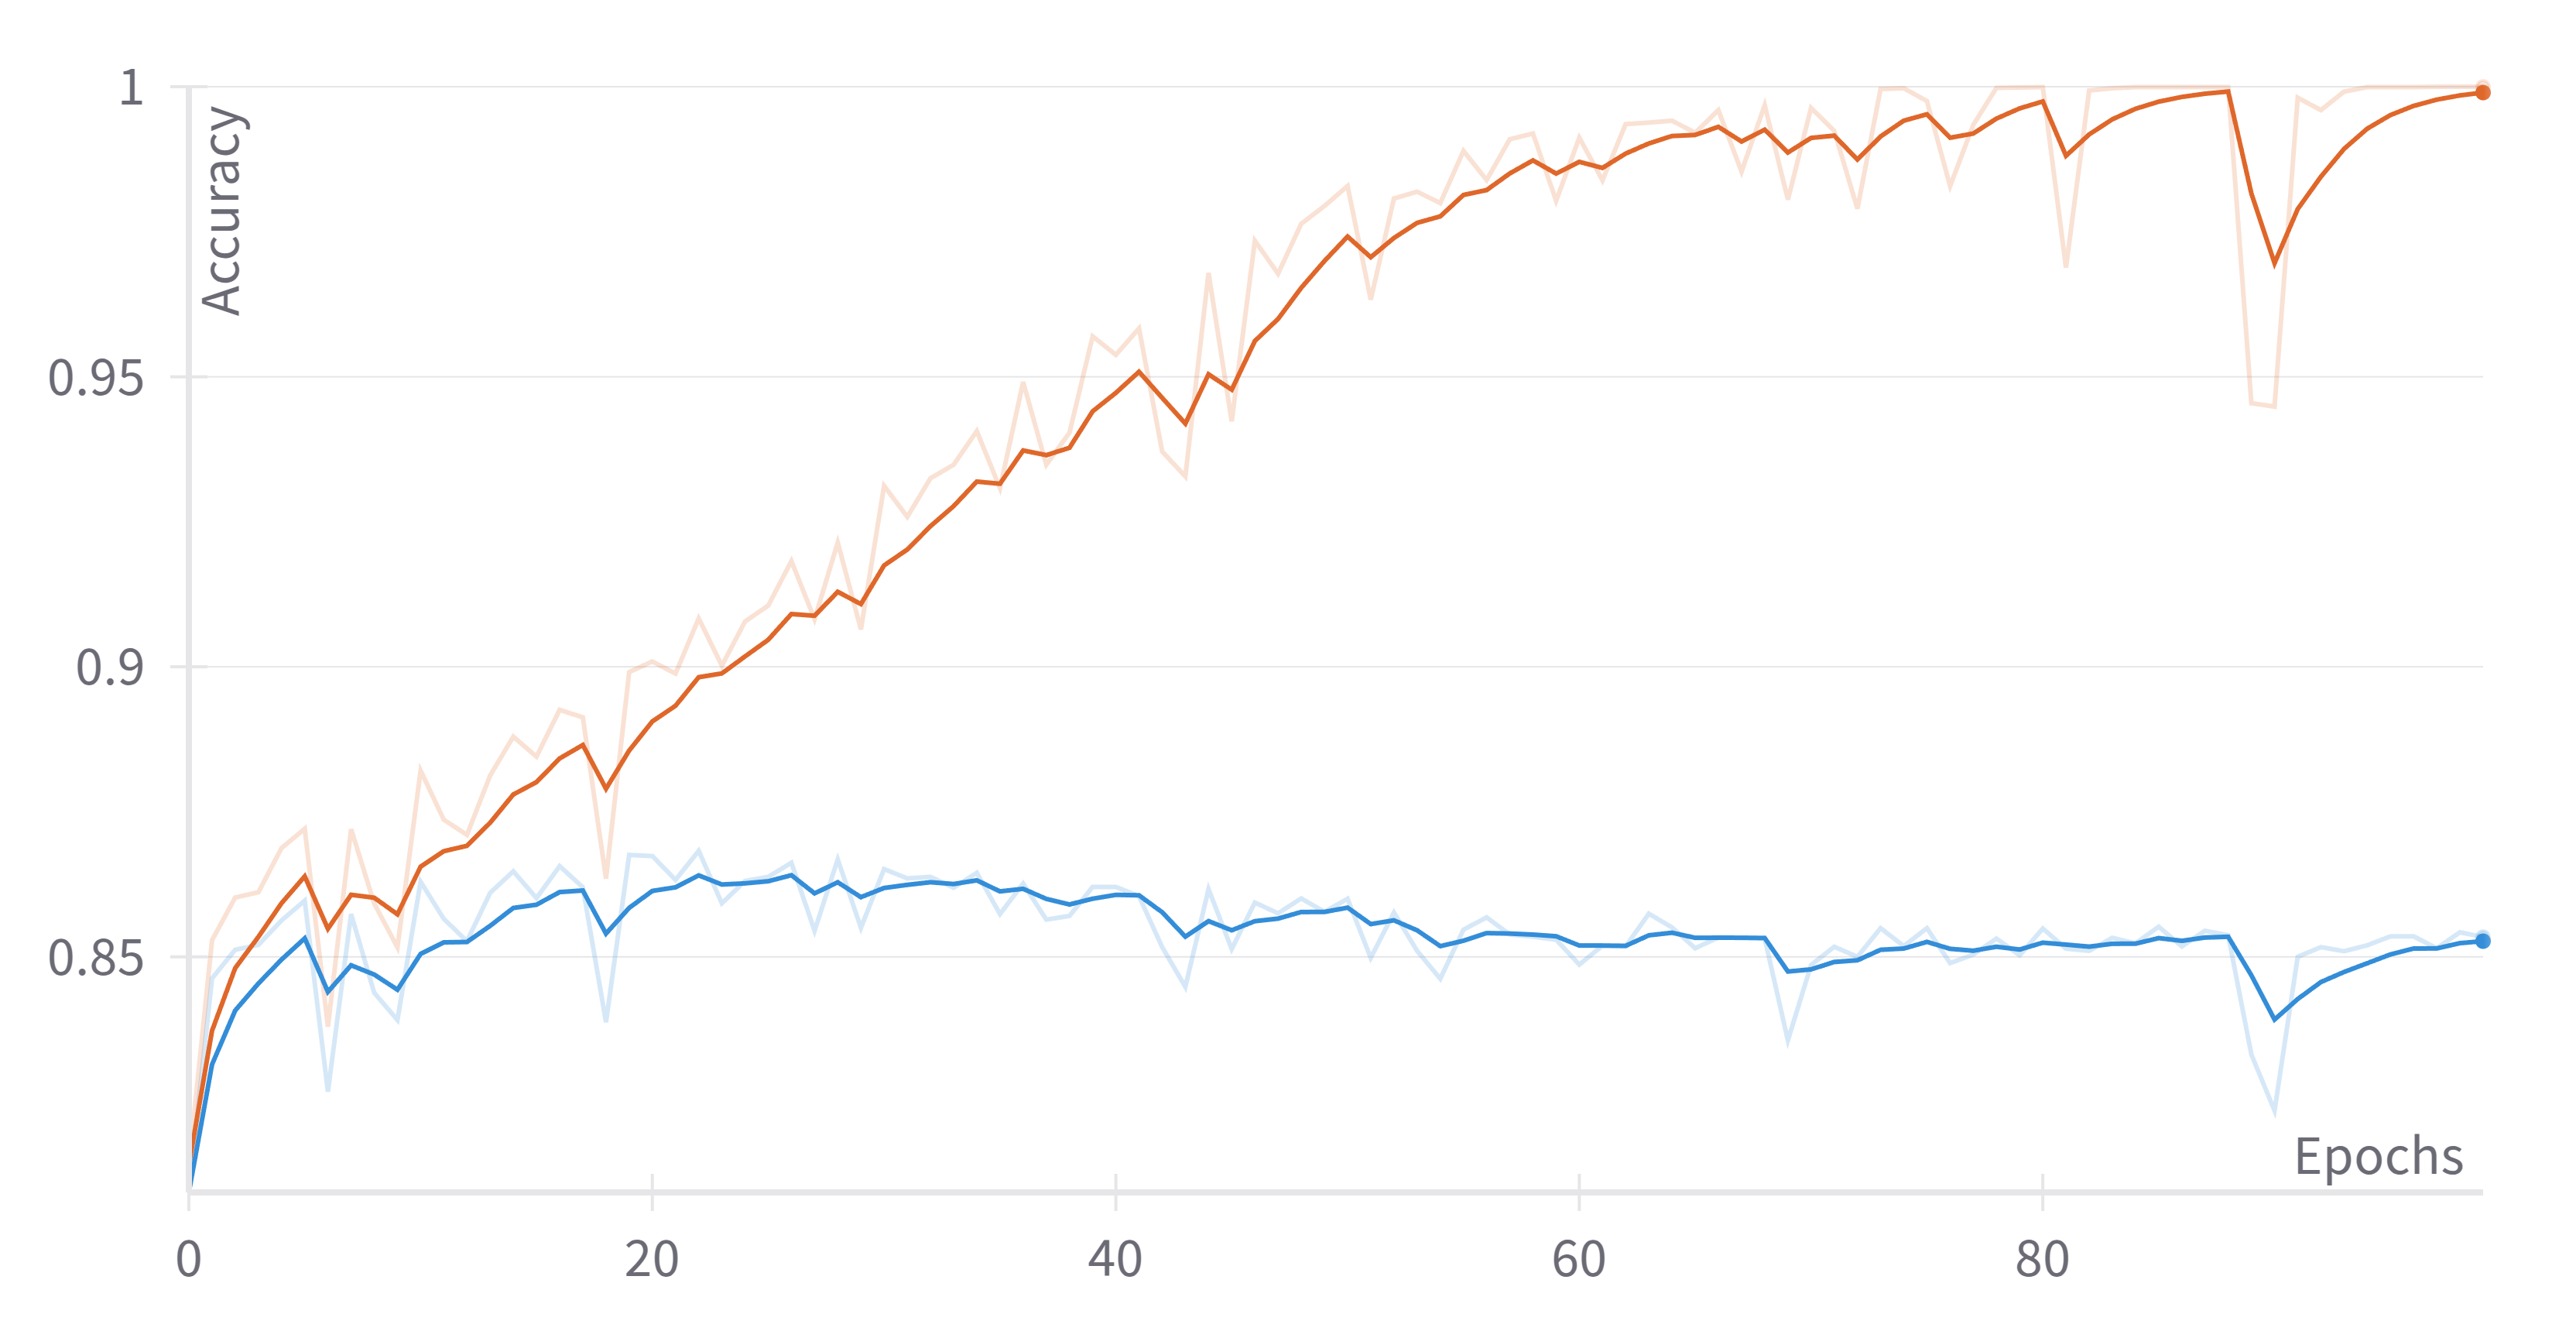
\includegraphics[width=\linewidth]{assets/pag/binary_classifier/baseline_overfitting.png}
        \caption{Baseline model: the training accuracy is $\approx 100\%$ while the validation is slowly downgrading}
    \end{subfigure}
    \hfill
    \begin{subfigure}{0.48\linewidth}
        \centering
        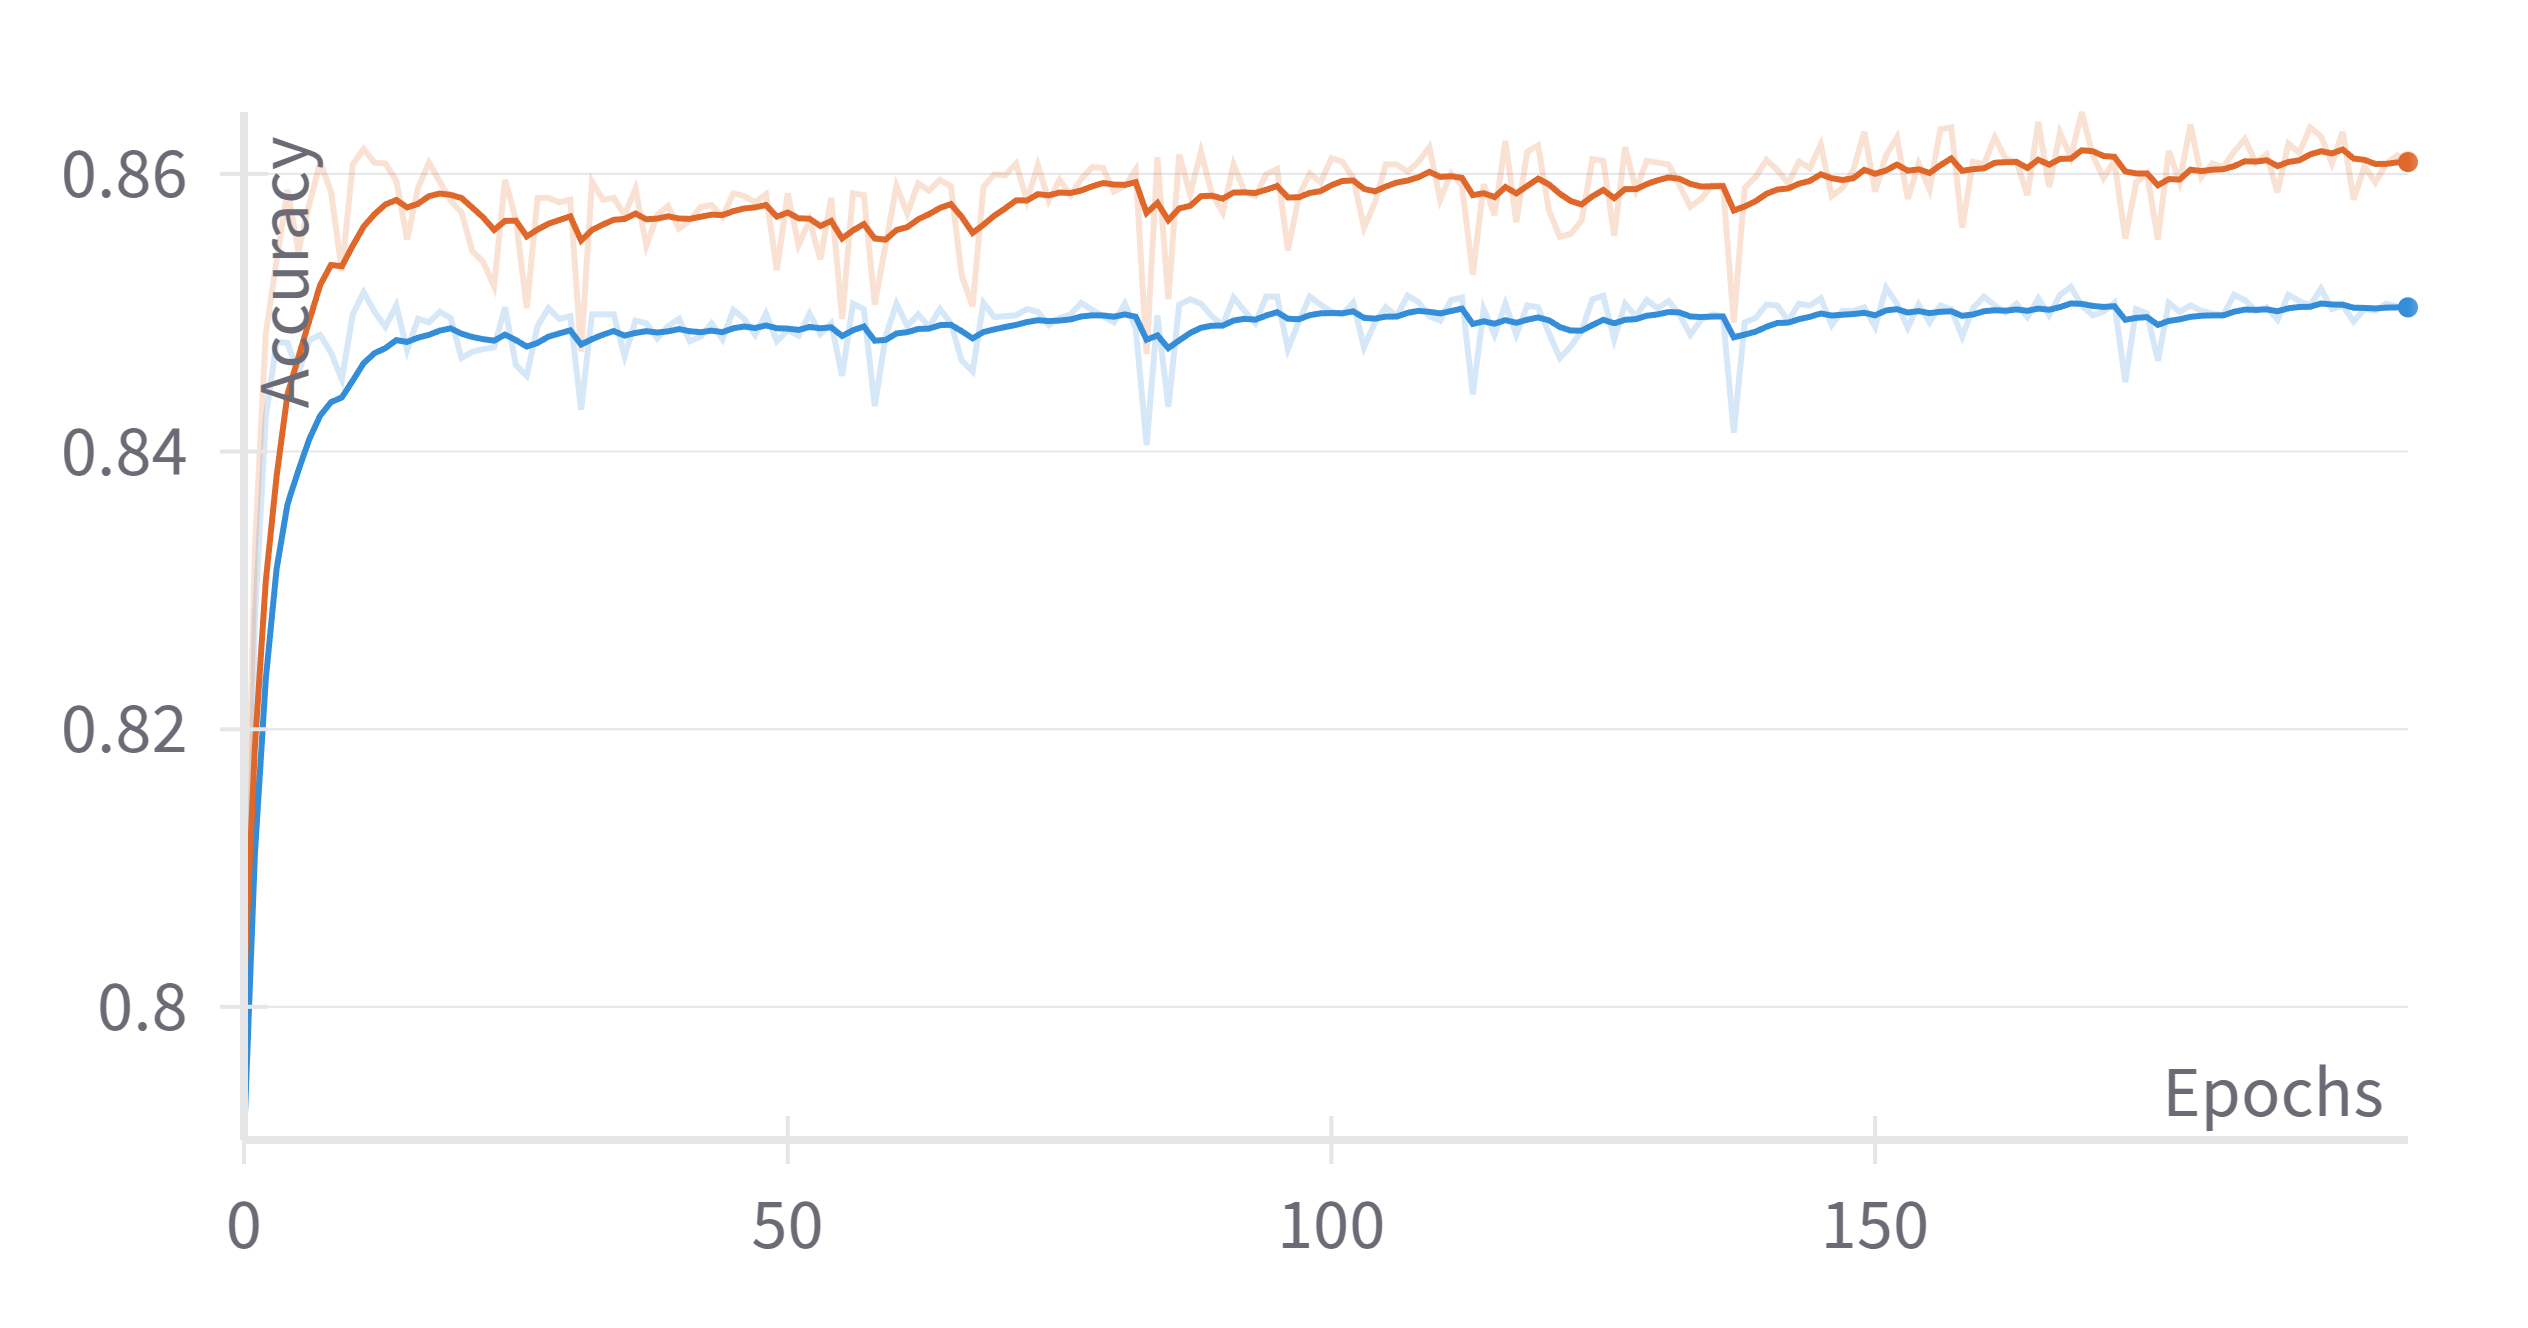
\includegraphics[width=\linewidth]{assets/pag/binary_classifier/pag_regular_accuracy.png}
        \caption{PAG-regularized model: the two accuracies do not diverge after twice the epochs}
    \end{subfigure}
    \caption{Regularization effect of the PAG-loss in terms of overfitting}
    \label{fig:pag_regularization_overfitting}
\end{figure}

A nice property of the PAG model we observed it is its resilience to overfitting:
keeping the same hyper-parameters and network architecture, it can be observed the baseline to overfit in almost 20 epochs, while the regularized model kept a stationary value for the train and test accuracy, both very similar between each other, even at the $200^\text{th}$ epoch, as observable in \cref{fig:pag_regularization_overfitting}.
This may be caused as an effect of the heavy \textbf{regularization} that doing a double backward pass introduces. Enforcing this, the $\nabla^2 \mathcal{L}$ is computed, providing to the optimizer a more complete picture of the loss landscape's geometry.
%%


\subsection{Robustness}
In order to test the robustness improvement using the PAG loss,
we compared it against the baseline model, having as the only differences the number of epochs and the presence/absence of the regularization term introduced by the PAG requirement.

In \cref{fig:pag__binary_sentences_fsgm} it can be noticed the difference in robustness against a simple FSGM attack with multiple values of $\alpha$.
In particular, in \cref{table:pag__binary_classifier_robustness}, the results of multiple attacks are reported. Some of them have been executed using the AutoAttack suite \citep{croce2020reliableautoattack}.
It's clear that the robustness improved by a lot in all tests, but the FSGM with a low value of $\alpha$, in which the baseline model was already quite robust, while the same cannot be told with high values of perturbations.
We are enforcing Perceptually Aligned Gradients by performing a \textbf{double backward pass}, introducing $\nabla_x$ in the loss. When we perform a double backward pass on a model, we are essentially computing second-order derivatives of the loss function with respect to the model parameters.
This allows the model to learn a smoother function and be more robust against adversarial attacks based on some perturbations $x'$ of the input $x$.


\begin{figure}[ht]
    \centering
    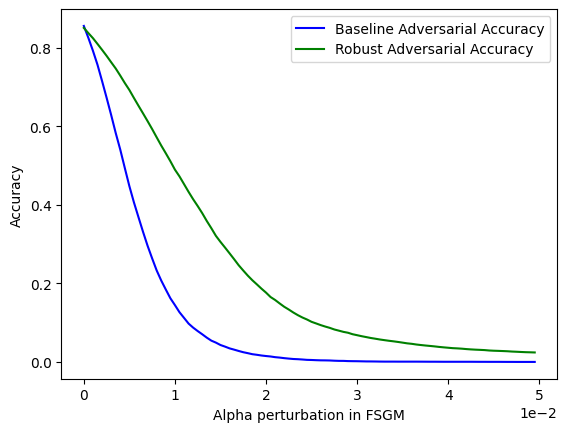
\includegraphics[width=0.5\linewidth]{assets/pag/binary_classifier/fsgm.png}
    \caption{Robustness against various $\alpha$ values in FSGM}
    \label{fig:pag__binary_sentences_fsgm}
\end{figure}

\begin{table}[ht]
\begin{tabular}{lcclccc}
\toprule
                             & \multicolumn{2}{c}{\textbf{APGD}}          & \textbf{Square}                     & \multicolumn{3}{c}{\textbf{FSGM}}                                                                               \\
                             & $\varepsilon = 1e-3$ & $\varepsilon = 0.5$ &                                     & \multicolumn{1}{l}{$\alpha = 1e-3$} & \multicolumn{1}{l}{$\alpha = 5e-3$} & \multicolumn{1}{l}{$\alpha = 1e-2$} \\
 \midrule
\multicolumn{1}{r}{Baseline} & 47.9\%               & 41.7\%              & \multicolumn{1}{c}{48.2\%}          & 79.2\%                              & 44.8\%                              & 14.5\%                              \\
\multicolumn{1}{r}{Robust}   & \textbf{75.8\%}      & \textbf{70.4\%}     & \multicolumn{1}{c}{\textbf{76.6\%}} & \textbf{82.4\%}                     & \textbf{69.2\%}                     & \textbf{49.0\%}                    \\
\bottomrule
\end{tabular}
\vspace{0.25cm}
\caption{Adversarial attacks comparing the two models}
\label{table:pag__binary_classifier_robustness}
\end{table}

The results in \cref{table:pag__binary_classifier_robustness} may be motivated by the following mental model.
When we apply a generic targeted gradient-based attack, generally we want to create the adversarial image with a perturbation derived from the gradients with respect to the input $x$.
The big change here is when these gradients actually present features of the target attack class.
From a high-level logical perspective, it can be seen as:

\begin{equation}
\begin{split}
    x' & = x + \alpha \nabla_x \mathcal{L}(x; y_\text{attack}; \theta) \quad \text{such that}\; y_\text{attack} \neq y_\text{true} \\
       & \approx x + \alpha (x_\text{attack} - x) \quad \text{since we minimize} \; d_{cos}(\nabla_x\mathcal{L}(x; y_\text{attack}), x_\text{attack} - x) \\
       &= x + \alpha \cdot x_\text{attack} - \alpha \cdot x \\
       &= (1 - \alpha) x + x_\text{attack}
\end{split}
\end{equation}

This small sketch of calculations can already highlight how the perturbed sample, when a classifier has Perceptually Aligned Gradients,
it is giving to the attack sample $x'$ the actual characteristics of a real sample of the target attack class.
It may be a mental model of the justification of why this approach gives more robustness, varying the value of $\alpha$ parameter.

Moreover, we can plot the activations of this classifier right before the Softmax function, to see how they are separated (\cref{fig:pag_pre_softmax_activations}).
Recall that this plot may be used as a certainty measure, where the more points are to the center, the more uncertainty there is.
Because of that, in our ideal scenario we have no point at the center, meaning maximum certainty in the prediction, which is unpractical but gives a measure of what the optimal solution may look like.

\begin{figure}
    \centering
    \begin{subfigure}{0.48\linewidth}
        \centering
        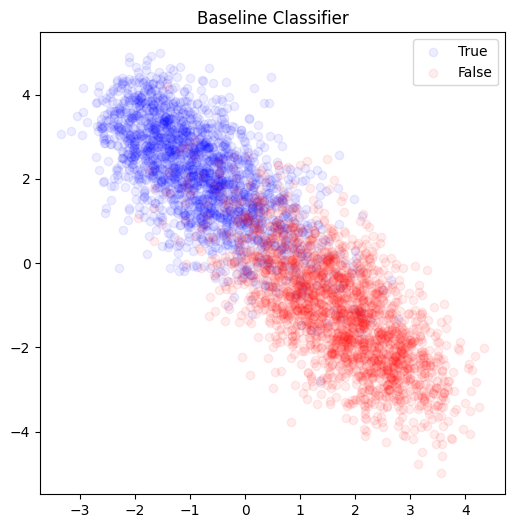
\includegraphics[width=\linewidth]{assets/pag/binary_classifier/pag_ce__baseline_softmax_activations.png}
        \caption{Baseline model: the point clouds are near each other}
    \end{subfigure}
    \hfill
    \begin{subfigure}{0.48\linewidth}
        \centering
        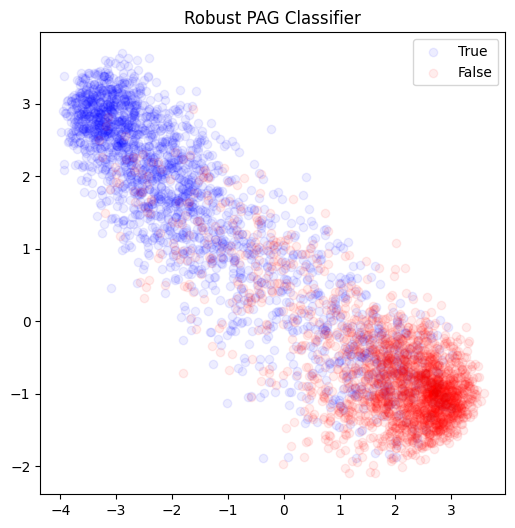
\includegraphics[width=\linewidth]{assets/pag/binary_classifier/pag_ce__robust_softmax_activations.png}
        \caption{PAG-regularized model: the point clouds are far from each other}
    \end{subfigure}
    \caption{Activations before softmax}
    \label{fig:pag_pre_softmax_activations}
\end{figure}

\subsection{PAG Variants}
\label{sec:pag__pag_variants_strategies}
We investigated how different PAG loss variants would affect the robustness and other metrics of this experiment.
We tested several models:
\begin{itemize}
    \item \emph{baseline}, with the Cross-Entropy loss only
    \item \emph{pag-score-similar-samples}, which implements the PAG formulation as in \cref{eq:pag_image_training_formula}
    \item \emph{pag-score-similar-features}, which computes the similarity of the transpose of the matrix previously mentioned, resulting in the input batch $\mathbf{X} \in \mathbb{R}^{N \times D}$, a set of random samples $\mathbf{G} \in \mathbb{R}^{N \times D}$, computing the PAG loss as $\mathcal{L}_{cos}(X^T, G^T)$ feature-wise, instead of comparing sample-wise, thus giving the name of this method
    \item \emph{pag-identity}, which imposes the $\nabla_x \mathcal{L}$ to be cosine-similar to $x$ itself
\end{itemize}

\subsubsection{Binary classifier}
When dealing with a binary classifier, we could observe that, on the contrary of our expectations,
the \emph{pag-score-similar-features} method is the one that works the best, with surprisingly good results (\cref{table:pag_variants_binary}), while not having any theoretical background to support it.

This led us to think again about this simplification of using a mere binary classifier, since it may be too small to let us explore the potential of Perceptually Aligned Gradients applied to text classification.

However, in the binary classification example, it is interesting to plot the logits of the classifier, before softmax, and see how they are placed in a 2D environment, changing the loss function, as can be seen in \cref{fig:pag_variants_logits_binary}.
It is worth remembering that the more distant the center of mass of the classes are, and the more certainty there is in their prediction by the classifier.

\begin{figure}[ht]
    \centering
    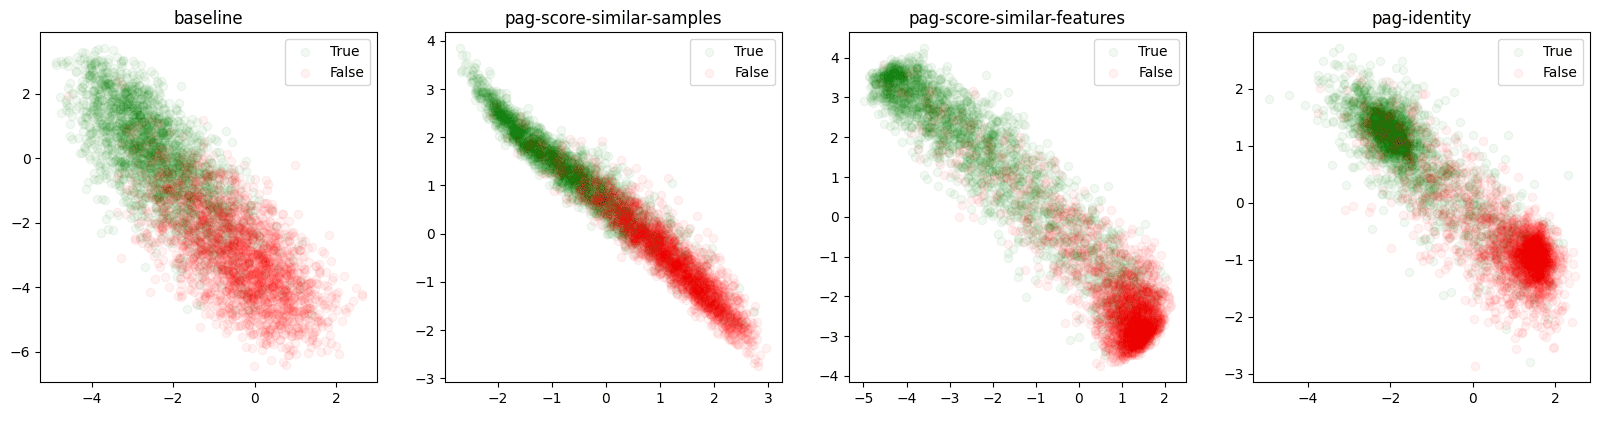
\includegraphics[width=\linewidth]{assets/pag/binary_classifier/logits.png}
    \caption{Logits of the binary classifier, according to the loss function used}
    \label{fig:pag_variants_logits_binary}
\end{figure}

\begin{table}[ht]
\resizebox{\textwidth}{!}{
\begin{tabular}{rcccccc}
\toprule
\multicolumn{1}{l}{}        & \multicolumn{2}{c}{\textbf{APGD}}          & \multicolumn{1}{l}{\textbf{Square}} & \multicolumn{3}{c}{\textbf{FSGM}}                                                                               \\
\multicolumn{1}{l}{}        & $\varepsilon = 1e-3$ & $\varepsilon = 0.5$ & \multicolumn{1}{l}{}                & \multicolumn{1}{l}{$\alpha = 1e-3$} & \multicolumn{1}{l}{$\alpha = 5e-3$} & \multicolumn{1}{l}{$\alpha = 1e-2$} \\
\midrule
Baseline                    & 47.9\%               & 41.7\%              & 48.2\%                              & 79.2\%                              & 44.8\%                              & 14.5\%                              \\
pag-scores similar-samples  & 57.0\%               & 42.7\%              & 56.5\%                              & 80.5\%                              & 68.1\%                              & 49.1\%                              \\
pag-scores similar-features & \textbf{71.8\%}      & \textbf{67.1\%}     & \textbf{73.1\%}                     & \textbf{81.7\%}                     & \textbf{71.4\%}                     & 55.3\%                              \\
pag-identity                & 43.5\%               & 43.1\%              & 43.8\%                              & \textbf{82.1\%}                     & 67.5\%                              & \textbf{56.4\%}                    \\
\bottomrule
\end{tabular}
}
\vspace{0.25cm}
\caption{Adversarial attacks comparing the PAG variants - \textbf{binary} classifier}
\label{table:pag_variants_binary}
\end{table}

\subsubsection{Multiclass classifier}
In order to have better understanding of the potential of applying PAG to text embeddings for classification,
we decided to introduce more entropy in the task, adding more classes.
To do that, we switch to a subset of the \texttt{amazon\_review\_multi} dataset (\citep{amazon-reviews-dataset}),
considering as classes the intersection of some languages (English, German, Spanish and French) and some reviews ratings (1, 3, 5), for a total of 12 classes, with 800 train samples each.
The embeddings are obtained as usual, taking the hidden state associated with the \texttt{[CLS]} token,
adopting the \texttt{distilbert-base-multilingual-cased} model
\footnote{\url{https://huggingface.co/distilbert/distilbert-base-multilingual-cased}}.
The models are trained using the same hyper-parameters, such as the $\lambda$ factors for the PAG regularization part of the loss, the number of epochs, and so on.

It finally gave us the results we expected, as observable now in \cref{table:pag_variants_multiclass}.
This highlights how the example of the binary classifier was just a random chance of having the right situation for the transpose cosine similarity to succeed, while in a more complex situation it does not work, as expected by the theoretical foundations and reasoning.


\begin{table}[ht]
\resizebox{\textwidth}{!}{
\begin{tabular}{rcccccc}
\toprule
\multicolumn{1}{l}{}        & \multicolumn{2}{c}{\textbf{APGD}}          & \multicolumn{1}{l}{\textbf{Square}} & \multicolumn{3}{c}{\textbf{FSGM}}                                                                               \\
\multicolumn{1}{l}{}        & $\varepsilon = 1e-3$ & $\varepsilon = 0.5$ & \multicolumn{1}{l}{}                & \multicolumn{1}{l}{$\alpha = 1e-3$} & \multicolumn{1}{l}{$\alpha = 5e-3$} & \multicolumn{1}{l}{$\alpha = 1e-2$} \\
\midrule
Baseline                    & 36.5\%               & 31.2\%              & 36.3\%                              & 60.3\%                              & 27.3\%                              & 8.9\%                               \\
pag-scores similar-samples  & \textbf{48.1\%}      & \textbf{45.0\%}     & \textbf{49.3\%}                     & \textbf{62.7\%}                     & \textbf{43.5\%}                     & \textbf{25.7\%}                     \\
pag-scores similar-features & 28.5\%               & 24.3\%              & 28.9\%                              & \textbf{62.3\%}                     & 40.1\%                              & 20.6\%                              \\
pag-identity                & 28.3\%               & 25.0\%              & 27.2\%                              & 60.1\%                              & 25.7\%                              & 8.0\%                              \\
\bottomrule
\end{tabular}
}
\vspace{0.25cm}
\caption{Adversarial attacks comparing the PAG variants - \textbf{multiclass} classifier}
\label{table:pag_variants_multiclass}
\end{table}

\section{Applying PAG to LLMs}
In the context of Large Language Models, it is not directly applicable the formulation of PAG as seen in \cref{eq:pag_image_training_formula} to LLMs.
The main issue is that an image is a continuous tensor that already contains all the information we need to clearly determine its predicted class.
In sequence processing this is not the case anymore, since the output will depend on the overall sequence instead of only just a single item or sample from it.
More importantly, the input tokens in the sequence are encoded are meaningless one-hot vectors.

This makes the gradient calculation on the input pretty challenging because:
\begin{itemize}
    \item calculating the gradients with respect to the input tokens does not provide the context of the overall sentence; to have a comparison with the image space, we can consider it as a single pixel, which of course cannot provide sufficient information about the input to determine the class (which is the next token in the sequence, in the context of an LLM)
    \item calculating the gradients with respect to an hidden state at a certain layer $i$ will require us to preload an index of possible hidden states for real sentences that have as a next token the one we want - this follows the vision of an LLM as a multiclass classifier over the last hidden state
    \item the number of classes to iterate on is huge, being the vocabulary size generally in the order of hundred of thousands of possible tokens; this makes the PAG loss applicable on images computationally infeasible when dealing with this order of magnitude of possible classes, thus entropy in the classification task.
\end{itemize}

An approach may be to approximate the PAG iteration over the classes, limiting our search to a restricted amount of classes, picking $K$ random next possible tokens among all the vocabulary $V$.
This will limit the computational resources required for the experiments, while also having the downside of not exploring possible directions for the gradients with some under-trained classes.

Multiple approaches can be considered when dealing with what to compute the gradients on, like the embedding vector of the single tokens or the hidden states of the sentence with respect to the last token in the sentence, which is the one that is more taken into account when predicting the next token during inference.

Consider:
\begin{itemize}
    \item the sample in the batch: $x_t$ = \texttt{the pen is on the}, with label $y_t$ = \texttt{table}
    \item a random sample: $x_t'$ = \texttt{using wood, you can build a}, with the same label $y_t$ = \texttt{table}
    \item another random sample: $x_f$ = \texttt{lot of trees form a}, with the label $y_f$ = \texttt{forest}
\end{itemize}

\begin{figure}
    \centering
    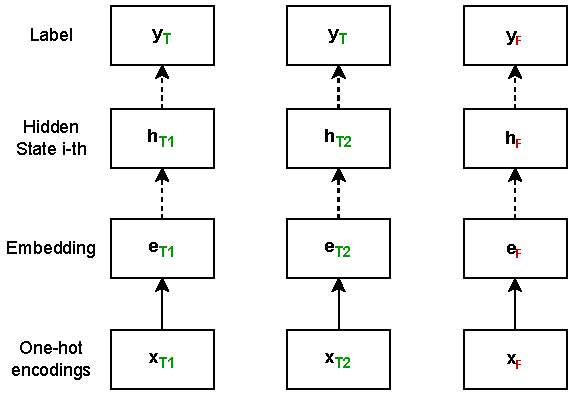
\includegraphics[width=0.7\linewidth]{assets/pag/llm/llm_hidden_states_sample_namings.drawio.pdf}
    \caption{Naming convention of the internal tensors of an LLM during a forward pass}
    \label{fig:llm_hidden_states_sample_namings}
\end{figure}

Following the naming scheme in the \cref{fig:llm_hidden_states_sample_namings},
we can compute the PAG loss in several different ways when dealing with text sequences.

\begin{equation}
\begin{split}
\mathcal{L}_\text{PAG}(x_t) & = d_{cos}(
\nabla_{e_t} \mathcal{L}_\text{CE}(x_t, y_t),
e_t' - e_t
) \\
& + d_{cos}(
\nabla_{e_f} \mathcal{L}_\text{CE}(x_t, y_f),
e_f - e_t
) \\
& + d_{cos}(\text{... over other classes ...})
\end{split}
\label{eq:pag_llm_embeddings}
\end{equation}

\begin{equation}
\begin{split}
\mathcal{L}_\text{PAG}(x_t) & = d_{cos}(
\nabla_{h_t} \mathcal{L}_\text{CE}(x_t, y_t),
h_t' - h_t
) \\
& + d_{cos}(
\nabla_{h_f} \mathcal{L}_\text{CE}(x_t, y_f),
h_f - h_t
) \\
& + d_{cos}(\text{... over other classes ...})
\end{split}
\label{eq:pag_llm_hidden_states}
\end{equation}

In the formulas above, the embedding refers to the last token, which is the one right before the predicted one.
The main point of this brief explanation is to show how it is not straightforward to try applying the well-known concept of PAG from images to discrete sequential text.
We may prefer to go down to the embedding layer (\cref{eq:pag_llm_embeddings}), where the notion of the overall sentence is absent, or staying in an intermediate hidden layer $i$ (\cref{eq:pag_llm_hidden_states}), even tough there are tons of other possible, unexplored in literature, alternatives. 

When dealing with gradients computed on the embeddings vectors we may think that they carry no information about the sentence, as the vector itself does not. However, it can be noticed that the gradients of the loss with respect to the embedding vector of a token $i$, contain information about both the past and the future tokens.
Indeed, in \cref{fig:llm_gradients_changing_embedding}, it is clear why the gradient on every embedding token of the full sentence is affected by the change of even only one input position, even keeping the labels unchanged.
The change of token $i$, influences its own logit prediction $i$ but also the future hidden states at time step $t: i < t \leq n$, because of the Masked self-attention layers present in every decoder transformer network.
The past tokens are also affected, even with masked self-attention. This can be explained using the chain rule of derivatives: the gradient of the loss with respect to an embedding will include in the equation also the partial derivative of the loss with respect to the affected logit $i$, thus changing the value of the gradient on the single embedding for $t: t < i$.
Note that: $\frac{\partial\mathcal{L}_i}{\partial{\text{logits}_i}} \propto \text{softmax}(\text{logits}_i)$, which are altered by the changed token $i$.

\begin{figure}
    \centering
    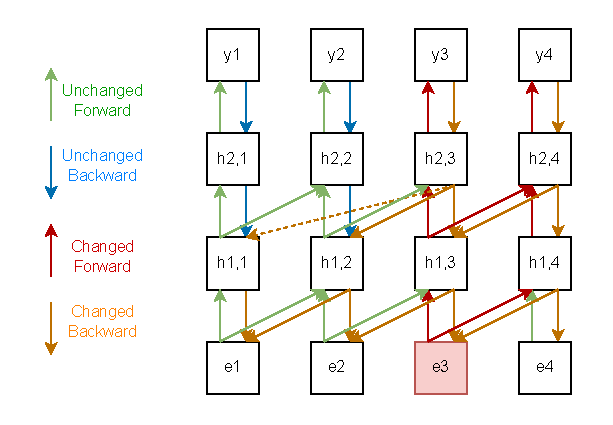
\includegraphics[width=0.7\linewidth]{assets/pag/llm/llm_gradients_changing_embedding.drawio.pdf}
    \caption{Simplification of gradients flow in an LLM changing only token $e_3$. In the forward pass, only future hidden states are affected. In the backward pass, the change propagates to every embedding token.}
    \label{fig:llm_gradients_changing_embedding}
\end{figure}

\subbib{}
\end{document}